\chapter{Integration by parts}
Chapter on asymptotic expansion of integrals. Many different special functions have ``integral representation''. For example, the Bessel function
\begin{gather*}
	J_0(x) = \frac{1}{\pi} \int_{0}^{\pi} \cos (x \sin t) \, \md t
\end{gather*}
which arises when solving, say, the wave equation on a circular drumhead (circular or cylindrical symmetry). The error function
\begin{gather*}
	\erf (x) = \frac{2}{\sqrt{\pi}} \int_{0}^{x} \me^{-t^2} \md t
\end{gather*}
arises when we look at probability or flow of heat/diffusion in 1D. The Gamma function
\begin{gather*}
	\Gamma(x) = \int_{0}^{\infty} t^{x-1} \me^{-t} \, \md t
\end{gather*}
generalizes the factorial (can interpolate between the integer factorials). \\
\ \newline
Often we solve linear ODEs and PDEs with transform (Laplace or Fourier) methods. These express the solution as an inverse transform, i.e. an integral. Asymptotics tell us the long-time ($t \gg 1$) or far-field ($x \gg 1$) behaviour of the solution. Useful when we cannot solve the integral in closed form. \\
\ \newline
\underline{Example:} Find the small-$x$ and large-$x$ expansions for
\begin{gather*}
	I(x) = \int_{x}^{\infty} \me^{-t^4} \md t \qquad x > 0
\end{gather*}
For small-$x$, can we expand the integral? This may be a good idea if the dominant contribution to the integral is coming from the region near $t = 0$. This will allow us to truncate early. However the series expansion to the exponential is still convergent and more generally we can write
\begin{align*}
	I(x) &= \int_{x}^{\infty} \left[1 - t^4 + \frac{t^8}{2!} - \dots \right] \md t
\end{align*}
However each term is divergent! Now they should all cancel term by term, to give us something finite, but that is not at all obvious using this approach. An alternative would be to split the problem into two integrals
\begin{align}
	I(x) &= \underbrace{\int_{0}^{\infty}}_{I_1} - \underbrace{\int_{0}^{x}}_{I_2} \nonumber \\
	&= \left({1}/{4}\right) \Gamma\left({1}/{4}\right) - \left(x - {x^5}/{5} + {x^9}/{18} - \dots \right) \label{eqn:smallx-limit}
\end{align}
\begin{itemize}
	\item where in order to evaluate the first integral $I_1$, with an exponential inside, we think in terms of the Gamma function and let $\tau = t^4$
	\item and the integral $I_2$ has been evaluated by integrating term by term
\end{itemize}
{\bf NB} The above series is convergent for \emph{all} $x$ but \emph{useless} for large $x$. Since, say for $x=10$, the numerator grows rapidly, and we would need an enormous number of terms before the denominator builds up enough to give decent convergence. \\
\ \newline
For large-$x$, we will try integration by parts:
\begin{align}
	I(x) &= \int_{x}^{\infty} \frac{\md (\me^{-t^4})}{-4t^3} \nonumber \\
	&= \underbrace{\frac{1}{4x^3} \me^{-x^4}}_{I_0(x)} \underbrace{- \frac{3}{4} \int_{x}^{\infty}  \frac{1}{t^4}\me^{-t^4} \md t}_{R(x)} \nonumber \\
	&= \frac{1}{4x^3} \me^{-x^4} - \frac{3}{16 x^7} \me^{-x^4} + \dots \label{eqn:largex-limit}
\end{align}
Note\footnote{We could have integrated by parts with the functions reversed, but that does not give us a series ordered in $1/x$.} that the remainder term $R(x) \ll I_0(x)$ because of the extra $1/t^4$ in the integrand and the fact that $t \geq x \gg 1$. In fact, we show that
\begin{gather*}
	I(x) \sim \frac{1}{4x^3} \me^{-x^4}
\end{gather*}
by estimating the size of the remainder term. 
\begin{align*}
	|R(x)| &= \frac{3}{4} \left|\int_{x}^{\infty} \frac{1}{t^4} \me^{-t^4} \md t \right| \\
	&= \frac{3}{16} \left|\int_{x}^{\infty} \frac{1}{t^7} {\md (\me^{-t^4})} \right| \\
	&< \frac{3}{16 x^7} \me^{-x^4}
\end{align*}
since $t>x$ in $t \in [x,\infty)$ implying $1/t^7 < 1/x^7$. The remainder term is less than the first term ignored in the series.

\begin{figure}[!h]
	\centering
	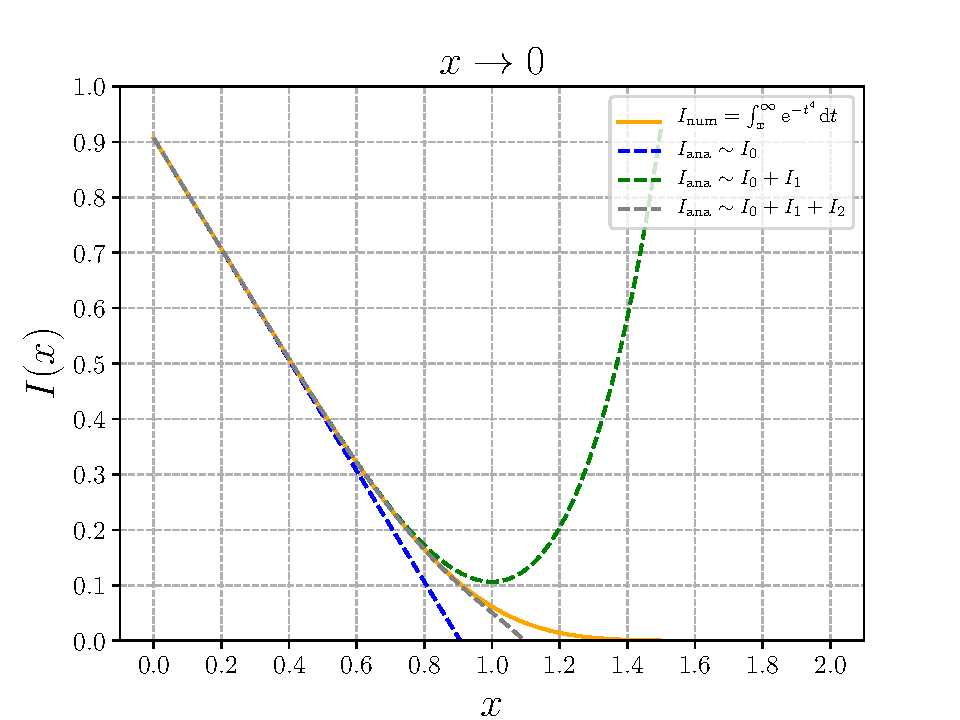
\includegraphics[width=0.9\textwidth]{./plots/pdf/strogatz-wk03-smallx.pdf}
	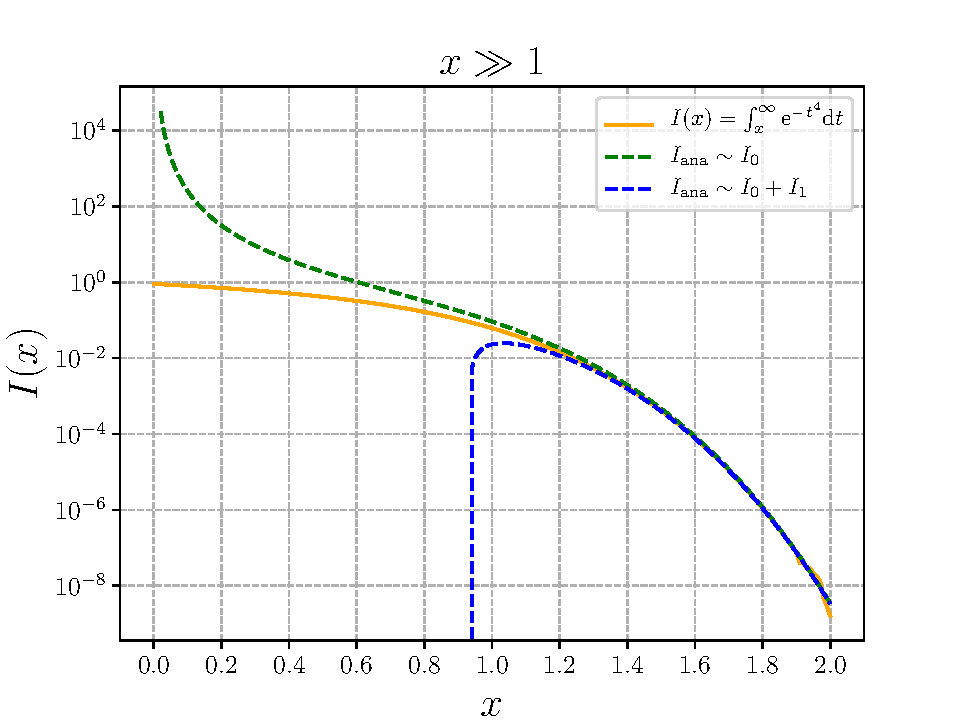
\includegraphics[width=0.9\textwidth]{./plots/pdf/strogatz-wk03-largex.pdf}
	\caption{Exact and asymptotic solutions to the integral in the small $x$ and large $x$ limits as given by the expressions \ref{eqn:smallx-limit} and \ref{eqn:largex-limit} respectively. }
	\label{fig:strogatz-wk03}
\end{figure}
\paragraph{General procedure for integration by parts on a Laplace integral}
\begin{align*}
	I(x) &= \int_{a}^{b} f(t) \me^{x \phi (t)} \md t \qquad x \rightarrow \infty \\
	&= \int_{a}^{b}  \frac{f(t)}{x \phi'(t)} \md (\me^{x \phi(t)}) \\
	&= \left. \frac{1}{x} \frac{f(t)}{\phi'(t)} \me^{x \phi(t)} \right|^b_a - \frac{1}{x}\int_{a}^{b} \left[\frac{f}{\phi'}\right]' \me^{x \phi(t)} \md t
\end{align*}
We need to assume
\begin{itemize}
	\item $\phi'(t) \neq 0$ anywhere inside the domain of integration; neither is $(f/\phi')'$
	\item $f(b)$ and $f(a)$ are not both zero
\end{itemize}
Further, if the second integral exists and is asymptotically smaller than the first term, then 
\begin{gather*}
	I(x) \sim \left. \frac{1}{x} \frac{f(t)}{\phi'(t)} \me^{x \phi(t)} \right|^b_a
\end{gather*}
\paragraph{NB} This method generates \emph{integer} powers of $1/x$. Will fail on problems where the correct asymptotics involve fractional powers of $x$ or $\log x$.
